\section{Evaluation}
\label{sec:eval}

Three questions. \textbf{RQ1} For each discipline, what does it prevent, and
what harm remains once it has? \textbf{RQ2} What does prevention cost, per
unit of work the discipline actually delivered? \textbf{RQ3} Where do the
structural preconditions of the anomalies occur in deployed code? A verified
arm's zero is a theorem, so every zero below is reported beside a count that
reads no runtime flag.

\smallskip\noindent\emph{Provenance.} Every table cell maps to a committed
trace directory and a scorer in the artifact; \texttt{reproduce.sh} rescores
all of them offline under an implementation of \cref{def:a1} independent of
the verified detector and the Rust port, and fails on any disagreement. The
numbers in this section were re-derived that way for this version.
Model-driven cells are one run each at the stated $n$; replicates differ by
model sampling, so a regeneration reproduces the protocol and the intervals,
not the sessions. Intervals are exact Clopper--Pearson unless stated.

\subsection{RQ1 on a live runtime: what $L_1$ removes and what it leaves}
\label{sec:live-a1}
The scenario of \cref{sec:intro-example} runs on an unmodified LangGraph
runtime (\texttt{langgraph} 1.2.0) with live models. Two compiled graphs
share one \texttt{BaseStore}, the framework's cross-thread memory, subclassed
only to stamp a logical clock at \texttt{get}/\texttt{put} under one lock;
\texttt{BaseStore} offers no version or compare-and-set, so the framework as
shipped cannot validate a read set. A flight agent reads the trip date,
drafts a reservation over a model call and puts the booking; a date agent,
started by the harness \LiveOffsetMs{}\,ms after the flight agent's read, reads
the date, asks its model for a one-week revision and puts it. Three modes:
\emph{vanilla}; \emph{validated}, the $L_1$ discipline at the application
layer (re-read before \texttt{put}, discard the generation and regenerate on
change); and \emph{sequential}, a control in which the date agent runs after
the flight agent commits. \LiveNPerCell{} sessions per cell on three model
families. Every session records the \A1 verdict on the emitted records, the
regenerations, the booking's date and the trip date at the end of the
session; \cref{tab:live} reports all four.

\begin{table*}[t]
\centering
\caption{Live cross-agent stale generation on an unmodified LangGraph runtime,
$n{=}100$ per cell at a $150$\,ms race offset; the date agent revises in every
session. \emph{\A1}: \cref{def:a1} on the emitted records. \emph{\Rp{}}:
\cref{def:residue} by argument provenance. \emph{Booking $\neq$ final}: the
harm, read off the store. \emph{Regen.}: discarded generations. Modes:
\emph{validated} is $L_1$ at the application layer; \emph{verified} takes
the commit decision from the verified $L_1$ store through a JSON bridge;
\emph{ledger} adds the basis ledger and a rebooking compensator. The first
three blocks' vanilla/validated/sequential rows are the committed September
run; the verified, ledger and deepseek-chat rows are an October run of all
four arms (its own vanilla/validated arms: $A_1=94$, $44$; residue $12$,
$51$), whose \Rp{} cells (``--'') are filled once its records pass the \Rp{}
gate---no cell is inferred as $100-A_1$.}
\label{tab:live}
\footnotesize
\setlength{\tabcolsep}{6pt}
\begin{tabular}{@{}llrrrr@{}}
\toprule
Model & Mode & \A1 (95\% CI) & \Rp{} & Booking $\neq$ final & Regen. \\
\midrule
\multirow{5}{*}{gpt-4o-mini}
 & vanilla    & $\LiveGptVanillaAOne/100$ [49.7, 69.7] & $\AsevenGptVanilla$ & $100/100$ & 0 \\
 & validated ($L_1$) & $0/100$ [0, 3.6] & $\AsevenGptValidated$ & $\LiveGptValidatedWrong/100$ [24.8, 44.2] & \LiveGptRegen \\
 & verified ($L_1$, verified store) & \LiveVerifiedGptAOne & \LiveVerifiedGptR & \LiveVerifiedGptWrong & \LiveVerifiedGptRegen \\
 & ledger ($L_1{+}\ell$) & \LiveLedgerGptAOne & \LiveLedgerGptR & \LiveLedgerGptWrong & \LiveLedgerGptRegen \\
 & sequential & $0/100$ [0, 3.6]  & $100$ & $100/100$ & 0 \\
\midrule
\multirow{5}{*}{claude-haiku-4-5}
 & vanilla    & $\LiveHaikuVanillaAOne/100$ [83.6, 95.8] & $\AsevenHaikuVanilla$ & $100/100$ & 0 \\
 & validated ($L_1$) & $0/100$ [0, 3.6] & $\AsevenHaikuValidated$ & $\LiveHaikuValidatedWrong/100$ [2.9, 13.9] & \LiveHaikuRegen \\
 & verified ($L_1$, verified store) & \LiveVerifiedHaikuAOne & \LiveVerifiedHaikuR & \LiveVerifiedHaikuWrong & \LiveVerifiedHaikuRegen \\
 & ledger ($L_1{+}\ell$) & \LiveLedgerHaikuAOne & \LiveLedgerHaikuR & \LiveLedgerHaikuWrong & \LiveLedgerHaikuRegen \\
 & sequential & $0/100$ [0, 3.6]  & $100$ & $100/100$ & 0 \\
\midrule
\multirow{3}{*}{Llama-3.2 (local)}
 & vanilla    & $\LiveLlamaVanillaAOne/100$ [0.0, 5.4] & $\AsevenLlamaVanilla$ & $100/100$ & 0 \\
 & validated ($L_1$) & $0/100$ [0, 3.6] & $\AsevenLlamaValidated$ & $\LiveLlamaValidatedWrong/100$ & 0 \\
 & sequential & $0/100$ [0, 3.6]  & $100$ & $100/100$ & 0 \\
\midrule
\multirow{4}{*}{deepseek-chat}
 & vanilla    & \LiveVanillaDeepseekAOne & \LiveVanillaDeepseekR & \LiveVanillaDeepseekWrong & \LiveVanillaDeepseekRegen \\
 & validated ($L_1$) & \LiveValidatedDeepseekAOne & \LiveValidatedDeepseekR & \LiveValidatedDeepseekWrong & \LiveValidatedDeepseekRegen \\
 & verified ($L_1$, verified store) & \LiveVerifiedDeepseekAOne & \LiveVerifiedDeepseekR & \LiveVerifiedDeepseekWrong & \LiveVerifiedDeepseekRegen \\
 & ledger ($L_1{+}\ell$) & \LiveLedgerDeepseekAOne & \LiveLedgerDeepseekR & \LiveLedgerDeepseekWrong & \LiveLedgerDeepseekRegen \\
\midrule
\multicolumn{6}{@{}l}{Pinned interval, read to commit, s (mean; max): gpt-4o-mini $\LiveGptPinnedMean$; $\LiveGptPinnedMax$ \quad haiku $\LiveHaikuPinnedMean$; $\LiveHaikuPinnedMax$ \quad Llama $\LiveLlamaPinnedMean$; $\LiveLlamaPinnedMax$}\\
\bottomrule
\end{tabular}
\end{table*}

\smallskip\noindent\textbf{The window is open and the framework does not
close it.} On both API models the runtime committed the stale booking in
every session in which the revision landed inside the window
($\LiveGptVanillaAOne\%$ and $\LiveHaikuVanillaAOne\%$), the detector fired
with the exact temporal witness of \cref{def:a1}, and in $150$ of those
$152$ firings the stale date reached the booking text; nothing in the
framework blocked, validated or reported any of them.

\smallskip\noindent\textbf{What the rates are.} Race outcomes: the
revision changed the value in $300/300$ sessions, and whether it landed
inside the window is the reviser's latency relative to the writer's plus the
fixed offset. The open-weights family makes this explicit: behind a
request-serializing local server the reviser's generation began only after
the flight agent's had finished, so the revision landed after the commit in
$99/100$ sessions and the one firing is the session with the longest pinned
interval ($\LiveLlamaPinnedMax$\,s). These are properties of the serving
configuration, not of the model or the framework.


\begin{figure}[t]
\centering
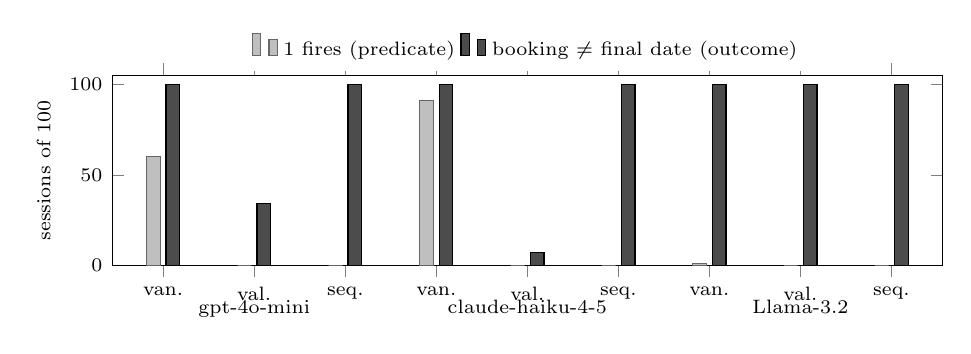
\begin{tikzpicture}
\begin{axis}[
  ybar, bar width=5pt, width=\columnwidth, height=4.0cm,
  ymin=0, ymax=105, ylabel={sessions of 100}, ylabel style={font=\scriptsize},
  symbolic x coords={gv,gp,gs,hv,hp,hs,lv,lp,ls},
  xtick=data, xticklabels={van.,val.,seq.,van.,val.,seq.,van.,val.,seq.},
  xticklabel style={font=\scriptsize}, yticklabel style={font=\scriptsize},
  legend style={font=\scriptsize, at={(0.5,1.02)}, anchor=south, legend columns=2, draw=none},
  enlarge x limits=0.07,
  extra x ticks={gp,hp,lp}, extra x tick labels={gpt-4o-mini, claude-haiku-4-5, Llama-3.2},
  extra x tick style={tick label style={yshift=-9pt,font=\scriptsize\itshape}, major tick length=0pt},
]
\addplot[fill=black!25,draw=black!60] coordinates {(gv,60) (gp,0) (gs,0) (hv,91) (hp,0) (hs,0) (lv,1) (lp,0) (ls,0)};
\addplot[fill=black!70,draw=black] coordinates {(gv,100) (gp,34) (gs,100) (hv,100) (hp,7) (hs,100) (lv,100) (lp,100) (ls,100)};
\legend{\A1 fires (predicate), booking $\neq$ final date (outcome)}
\end{axis}
\end{tikzpicture}
\caption{Predicate against outcome in the live study (\cref{tab:live}). The
$L_1$ discipline (\emph{val.}) drives the predicate to zero; the outcome it
leaves is the post-commit supersession, which the sequential control
(\emph{seq.}) exhibits in every session while satisfying every predicate.}
\label{fig:outcome}
\end{figure}

\smallskip\noindent\textbf{What $L_1$ removes, and what it does not.}
Read-set validation removed every firing ($0/300$) at one discarded
generation per realized conflict (\LiveGptRegen{} and \LiveHaikuRegen{} per
$100$ sessions, never two in one session, none where the race never
realized). It did not make the booking agree with the final trip date: in
$\LiveGptValidatedWrong$ and $\LiveHaikuValidatedWrong$ of $100$ sessions the
revision landed after the commit, the committed record is current at its
commit point exactly as \cref{thm:corc} says, and the booking is stale with
respect to a state that did not yet exist. That residue is a post-commit
supersession---the blind overwrite of \cref{sec:a1}, serializable in commit
order, outside every isolation discipline---and it is the shape the $L_2$
question addresses from the other side: the booking is an externalized
effect whose basis was later withdrawn, and only compensation (or holding the
effect until the basis is final) reaches it. On this workload $L_1$ buys
exactly commit-order read consistency; the \emph{sequential} control, clean
under every commit-time predicate, delivers the wrong booking in $100/100$
sessions for the same reason. Reporting the predicate alone would have
credited $L_1$ with a correctness it does not provide (\cref{fig:outcome}).

\smallskip\noindent\textbf{\Rp{} decides the residue on the records.}
\Cref{def:residue} names what is left, and the \Rp{} column of
\cref{tab:live} is decided on the emitted records alone: the basis of each
booking is the date value in its arguments, and \Rp{} fires in exactly the
sessions whose booking disagrees with the final date and \A1 does not
($A_1+R=100$ in every unguarded cell; under $L_1$ the \Rp{} column equals
the residue; \texttt{a7\_rescore.py -{}-check}). The identity is between two
independent computations (\cref{sec:residue}), and it holds here because
the booking tool takes the date as a structured argument; a workload whose
effects paraphrase their inputs would show a recall below
\HypBasisRecovered/\HypBookings{} and a smaller \Rp{} column, never a larger
one. Two further arms run the same harness on three API families (haiku,
gpt-4o-mini and deepseek-chat, the last through its OpenAI-compatible
endpoint). In the \emph{verified} arm the $L_1$ decision is taken by the
verified store through the bridge of \cref{sec:trust}: \A1 fires in $0/300$
sessions, and the residue is $2$, $51$ and $52$ of $100$---the same kind of
number the application-layer arm leaves in the same run ($12$, $51$, $63$),
the haiku pair differing by run-to-run sampling of which revisions land
after the commit; the two runs of the validated arm on gpt-4o-mini ($34$ in
September, $51$ in October) show the same spread across runs, which is why
the offset sweep repeats every cell.
In the \emph{ledger} arm a superseding put registers the obligation and a
compensator issues a replacement booking: the outcome column is $0/100$ on
all three families, at the price of the discarded generations of $L_1$ plus
one compensation generation per registered obligation. What
\cref{prop:owed} says must remain after release does remain under every
commit-time discipline, and the ledger is the one arm that answers it.

\smallskip\noindent\textbf{Superstep.} A second graph places a writer and a
summarizer of one reducer-declared channel in one Pregel
superstep~\cite{MalewiczEtAl2010Pregel}; the barrier hands both the snapshot
at superstep entry, so in $300/300$ sessions the summary names the
destination the writer had changed. This is the snapshot-insufficiency shape
of \cref{sec:snapshot} observed live---a reducer buys lost-update freedom,
not $L_1$---reported as documented BSP semantics, not as a rate: the census
finds the shape in no public graph, and under a completion clock
\cref{def:a1} fires exactly when the writer's body returned first
(\SuperstepGpt, \SuperstepHaiku, \SuperstepLlama{} of $100$;
\texttt{check\_clocks.sh}).

\ifnum\OffsetCurveAvailable=1 \begin{figure}[t]
\centering
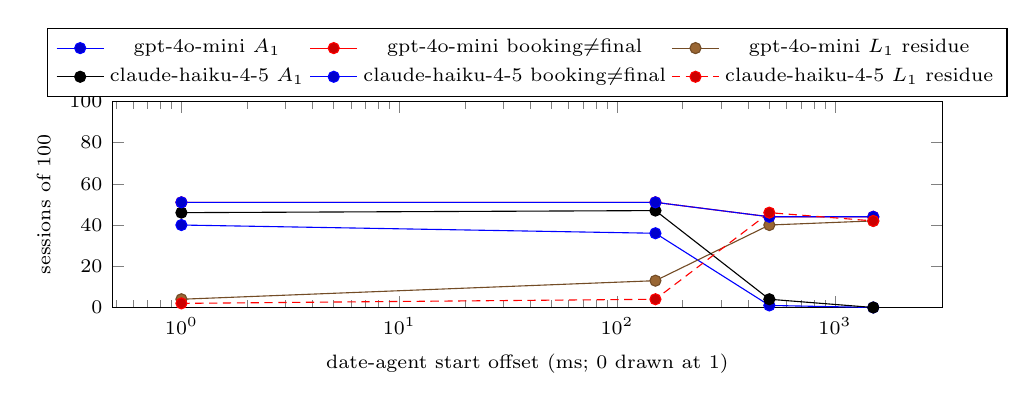
\begin{tikzpicture}
\begin{axis}[width=\columnwidth, height=4.2cm, xmode=log, log basis x=10, xlabel={date-agent start offset (ms; 0 drawn at 1)},
  ylabel={sessions of 100}, ymin=0, ymax=100, legend style={font=\scriptsize, at={(0.5,1.02)}, anchor=south, legend columns=3}, tick label style={font=\scriptsize}, label style={font=\scriptsize}]
\addplot+[mark=*] coordinates {(1,40) (150,36) (500,1) (1500,0)};
\addlegendentry{gpt-4o-mini $A_1$}
\addplot+[mark=*] coordinates {(1,51) (150,51) (500,44) (1500,44)};
\addlegendentry{gpt-4o-mini booking$\neq$final}
\addplot+[mark=*] coordinates {(1,4) (150,13) (500,40) (1500,42)};
\addlegendentry{gpt-4o-mini $L_1$ residue}
\addplot+[mark=*] coordinates {(1,46) (150,47) (500,4) (1500,0)};
\addlegendentry{claude-haiku-4-5 $A_1$}
\addplot+[mark=*] coordinates {(1,51) (150,51) (500,44) (1500,44)};
\addlegendentry{claude-haiku-4-5 booking$\neq$final}
\addplot+[mark=*] coordinates {(1,2) (150,4) (500,46) (1500,42)};
\addlegendentry{claude-haiku-4-5 $L_1$ residue}
\end{axis}
\end{tikzpicture}
\caption{Probe 303: the live \A1 rate and the outcome as a function of the date agent's start offset (revision probability $0.5$; $n=100$ per cell).}
\label{fig:offset}
\end{figure}
\fi

\subsection{RQ1 across three disciplines: the AutoGen pilot}
\label{sec:pilot}
An instrumentation layer exposes a two-phase \texttt{begin}/\texttt{commit}
API to LLM-driven agents under AutoGen~\cite{WuEtAl2023AutoGen}; the Rust
runtimes of \cref{sec:l1} sit behind it. Three workloads span the space from
concurrent to sequential: \emph{edit-review} (two agents both read
\texttt{doc} before either writes---overlap forced), \emph{plan-execute}
(strictly sequential---overlap forbidden) and \emph{triage} (a three-agent
pipeline whose overlap is left to the models). gpt-4o, $100$ sessions per
cell, three runtimes (\cref{tab:pilot}); the vanilla column was replicated
three times (triage \PilotTriageRates; pooled \PilotTriagePooled).

\begin{table}[t]
\centering
\caption{AutoGen pilot, \A1 firing rate by runtime and workload (run
\texttt{\CostRun}, $n{=}100$ per cell). \emph{Complete \& clean}: sessions
with no \A1 witness in which every role that commits in the unguarded cell
also commits here.}
\label{tab:pilot}
\footnotesize
\setlength{\tabcolsep}{3pt}
\resizebox{\columnwidth}{!}{%
\begin{tabular}{@{}lccc@{}}
\toprule
Runtime & edit-review & plan-execute & triage \\
\midrule
Vanilla & 100\% [96.4, 100] & 0\% [0, 3.6] & 48\% [37.9, 58.2] \\
Pessimistic locking & 0\% [0, 3.6] & 0\% [0, 3.6] & 0\% [0, 3.6] \\
Snapshot isolation (default-SI) & \PilotSiEditResidual\% [1.6, 11.3] & 0\% [0, 3.6] & \PilotSiTriageResidual\% [3.5, 15.2] \\
\midrule
Complete \& clean, vanilla / pess. / SI & 0 / 1 / 0 & 99 / 100 / 99 & 52 / 3 / 45 \\
\bottomrule
\end{tabular}}
\end{table}

Both endpoints are engineered, so the table is a sensitivity check of the
detector and the runtimes on model-driven traces, not a prevalence. Every
edit-review witness is a cold-start read (the reviewer read the document
before the editor's first write landed), unlike the live study's
supersessions.
Default-SI's residual is its no-write bypass: a read-only commit is never
validated, which is the classical write-only SI behavior and the unfaithful
emitter of Theorem L1j; SSI mode closes it. Pessimistic locking reaches
$0\%$ on edit-review by refusing the reviewer's operation in $99/100$
sessions---the anomaly is absent because the work is---and on triage by
dropping one of three agents in $97/100$. The \emph{complete \& clean} row is
the number to read a prevention claim against, and on triage it favors the
unguarded baseline ($52$) over default-SI ($45$) and pessimistic locking
($3$), because default-SI drops the engineer in $47\%$ of sessions and
pessimistic locking in $97\%$. Whether a dropped contribution or a stale one
is the worse outcome is a property of the task, not of the discipline, and
is why \cref{sec:cost} prices prevention per sound committed operation.

\subsection{RQ1 for $L_2$: output commit on synthetic cascades and live verdicts}
\label{sec:l2-eval}
Three arms run the same $1{,}000$ seeded schedules at nominal chain depths
$2$, $3$ and $5$: a root commits, a chain of dependents reads the previous
cell and commits, one committed transaction is put under review and retracted
or approved, and in a quarter of scenarios the review arrives after that
transaction has released. The \emph{verified} arm is \texttt{l2\_exec.rs};
the \emph{unguarded} arm validates reads, releases at commit and flags only
the aborted transaction; the \emph{cascade} arm releases at commit and
cascades the abort. Each trace is scored under \cref{def:a3}, under the
surviving-dependent predicate, and by \emph{exposed effects}---effects out at
the end although the review asked to withdraw their basis---which reads no
flag (full table: supplement \S\,P). The result is one structural fact.
\Cref{def:a3} fires in \LtwoDefThreeBaseline{} of $1{,}000$ schedules per
depth under both baselines and in none under the verified arm; the cascade
arm satisfies its own surviving-dependent predicate in every scenario while
exposing exactly as many effects as no discipline at all
(\LtwoExposedBaseline{}), because it flagged \LtwoRelabeled{} dependents
\emph{after} their effects were out---a cascade without output commit moves
flags, not effects. The verified arm is not zero on exposed effects:
\LtwoExposedVerified{} effects in $199$ scenarios per depth, exactly the
scenarios in which the review arrived after the release and the retraction
was refused. The figures decompose by arithmetic ($1{,}538 = 402 + 572 +
564$ at depth 2): the first term no runtime can remove; the second, one
reviewed operation per early review, any runtime that declines to release an
operation under review avoids; the third ($37$--$46\%$ of the unguarded
exposure) is output commit's own contribution, dependents whose release it
refused and the cascade then cancelled. Its cost is delay, not liveness:
$748$, $1{,}255$ and $1{,}272$ operations had a release refused at least
once, and every committed-and-unaborted operation was eventually released.
The quarter of late reviews is a harness parameter, so the overall exposure
reduction ($73$--$74\%$) is that parameter seen from the other side and is
not a finding.

\smallskip\noindent\textbf{Live verdicts.} A plan--execute--revise workload
driven by real models (a planner commits a plan; an executor reads it,
acquiring the planner as predecessor, and commits; a supervisor decides from
the ticket and plan whether to retract) was recorded for $200$ sessions on
each of three families and replayed through the three arms. Retraction rates
varied sharply---$1/200$ (claude-haiku-4-5), $3/200$ (gpt-4o-mini),
$62/200$ (Llama-3.2)---so we make the pooled statement only: in every one of
the \LiveLtwoRetractions{} retracted sessions the unguarded baseline and the
cascade design left a \cref{def:a3} witness (the latter while satisfying the
surviving-dependent predicate), and the verified runtime released no executor
effect on a retracted plan, at a pooled release rate of $89.0\%$. The zero is
structural; what the replay adds is that the discipline executes under
divergent live supervisor behavior at a stated cost.

\subsection{RQ1 for $L_3$: a released tool executor reorders}
\label{sec:a6-eval}
LangGraph's \texttt{ToolNode} dispatches a turn's tool calls concurrently
(\texttt{asyncio.gather}), collects results in input order and does not
serialize side effects; its tracker records a user needing sequential
execution for stateful tools and unable to obtain it (langgraphjs \#861). We
gave three backbones a natural prompt (no instruction to parallelize) over
five order-dependent infrastructure tools whose docstrings state their
dependencies, took the model-emitted call list as $\fld{io}$, and dispatched
it through the released \texttt{ToolNode} and through the $L_3$ sequencer.
In the table's cells two things are real---whether a backbone batches an
order-dependent pipeline into one turn, and the executor---and per-tool
latency is modeled, drawn uniformly from $10$--$200$\,ms (a uniform-latency
control produces no reorder; the committed order is the latency argsort).
The replay against real effects below removes the model.

\begin{table}[t]
\centering
\caption{Model-emitted batches through LangGraph's released \texttt{ToolNode}
(\texttt{langgraph} 1.2.5), $30$ turns per backbone, natural prompt. Tool
latency modeled. \emph{Transcript}: turns in which the returned
\texttt{ToolMessage} list preserved issuance order although effects committed
out of order.}
\label{tab:toolnode}
\footnotesize
\setlength{\tabcolsep}{3pt}
\resizebox{\columnwidth}{!}{%
\begin{tabular}{@{}lcccc@{}}
\toprule
Backbone & batched & full pipeline (5) & \A6, default & \A6, $L_3$ \\
\midrule
gpt-4o-mini & \ToolNodeGptBatched/30 & \ToolNodeGptFull{} (\ToolNodeGptFull{} reordered) & \ToolNodeGptReordered/\ToolNodeGptBatched & 0/\ToolNodeGptBatched \\
Llama-3.2 & \ToolNodeLlamaBatched/30 & 0 & \ToolNodeLlamaReordered/\ToolNodeLlamaBatched & 0/\ToolNodeLlamaBatched \\
claude-haiku-4-5 & 0/30 & 0 & --- & --- \\
\midrule
\multicolumn{5}{@{}l}{Transcript preserved issuance order in \ToolNodeBatchedTurns/\ToolNodeBatchedTurns{} batched turns; \ToolNodeReorderings{} of them had committed out of order.}\\
\bottomrule
\end{tabular}}
\end{table}

The finding that survives the modeling is structural
(\cref{tab:toolnode}): one backbone batches the full dependent pipeline on
$\ToolNodeGptFull/30$ turns and reorders every one of them, another never
batches, and the transcript a developer inspects shows the correct order in
all \ToolNodeBatchedTurns{} batched turns while the external state does not.
Calls emitted in one turn are, by the provider's contract, calls the model
declared parallelizable, so the defect is shared between a backbone that
misjudged independence and an executor that cannot notice; the $L_3$
sequencer makes effect order independent of which backbone is in use, which
is the property the cross-model spread shows cannot otherwise be assumed.
Replaying the $33$ recorded batches five times each through
\texttt{ToolNode} against real effects---a WAL-backed SQLite database and a
local HTTP service, with whatever latency those have---rather than a modeled
sleep, baseline \A6 fires in \ToolNodeRealSqlite{} replays (SQLite) and
\ToolNodeRealHttp{} (HTTP), and $L_3$ in none: the reorder is a property of
concurrent dispatch under any real latency, not of the distribution we drew.

\subsection{RQ1 for $L_4$: validation at dispatch}
\label{sec:l4-eval}
One seeded schedule per run pins a tool and then revokes or re-signs random
tools; three dispatchers act on the same registry. Over $1{,}000$ runs at
registry widths $2$, $4$ and $16$ the churn touched the planned tool in
\LfourPhantom{} runs, and in exactly those runs both live resolution and
snapshot resolution called a phantom---Theorem $L_4$d measured rather than
argued---while the verified dispatcher (\texttt{l4\_exec.rs}, the verified
bytes) called none and refused exactly those runs. The informative figures
are the hazard rate and the refusal cost; the zero is Theorem $L_4$b
executing.

\subsection{RQ2: what prevention costs}
\label{sec:cost}
The pilot driver captures per-call usage and wall-clock for every session of
run \texttt{\CostRun} (gpt-4o, $900$ sessions) and of its Claude Sonnet~4.5
replication; pricing is list price at the time of the run. Per session,
snapshot isolation's token cost is not separable from the unguarded
runtime's on either provider (overlapping intervals in every cell), and
pessimistic locking's overhead is bounded but provider-dependent (at most
$1.6\times$ on gpt-4o and $2.3\times$ on Claude, both on triage, where it
retries). A per-session denominator, however, credits a discipline for work
it declined to do. \Cref{tab:cost} re-prices the same run per committed
operation and per \emph{sound} committed operation---one that is not the
stale reader of any \cref{def:a1} witness---so that no runtime earns credit
for output an anomaly has invalidated.

\begin{table}[t]
\centering
\caption{Token cost of prevention under three denominators, gpt-4o, run
\texttt{\CostRun}. Per sound committed operation is the price we recommend
reading. Underlying counts (commits / sound): edit-review vanilla $212/112$,
pessimistic $101/101$, SI $110/105$; triage vanilla $335/283$, pessimistic
$205/205$, SI $268/256$; plan-execute $\approx200/200$ for all three.}
\label{tab:cost}
\footnotesize
\setlength{\tabcolsep}{3.5pt}
\resizebox{\columnwidth}{!}{%
\begin{tabular}{@{}llrrr@{}}
\toprule
Workload & Discipline & per session & per commit & per sound commit \\
\midrule
edit-review  & pessimistic & $+3.8\%$  & $+117.9\%$ & $+15.1\%$ \\
edit-review  & SI          & $+0.6\%$  & $+94.0\%$  & $+7.4\%$  \\
plan-execute & pessimistic & $+1.7\%$  & $+1.2\%$   & $+1.2\%$  \\
plan-execute & SI          & $+0.4\%$  & $+0.4\%$   & $+0.4\%$  \\
triage       & pessimistic & $+42.7\%$ & $+133.2\%$ & $+97.0\%$ \\
triage       & SI          & $+0.5\%$  & $+25.6\%$  & $+11.1\%$ \\
\bottomrule
\end{tabular}}
\end{table}

Between-session parity does not survive the change of denominator: snapshot
isolation costs $+7.4\%$, $+0.4\%$ and $+11.1\%$ per sound committed
operation, and pessimistic locking's triage penalty is $+97\%$ rather than
$+43\%$. Overhead tracks realized contention: edit-review, which aborts
hardest, pays most; plan-execute, which never aborts, pays nothing under any
denominator. A separate $155$-session paired sweep on gpt-4o-mini (fan-in
$2$--$16$ at one cell; $2$--$32$ cells at fan-in $8$; realized abort rates
$0.09$--$0.93$) resolves the mechanism: snapshot isolation carries no fixed
overhead (intercept $+0.05\%$, CI $[-1.5,+1.7]$) and pays $1.074\times$
$[1.052, 1.096]$ a first-attempt generation per abort, because the retry
carries the conflict into its prompt; the per-abort price does not steepen
with contention (supplement \S\,M).

\smallskip\noindent\textbf{Wall-clock, with its confound.} The nine cells of
a run were executed one after another, so a difference between cells carries
whatever the provider's latency did in between. Plan-execute, on which no
runtime aborts, is the control, and its ``overheads'' are $-4.5\%$ and
$-4.9\%$ on gpt-4o (Holm-corrected permutation $p=0.014$, $0.002$) and
$+13.5\%$ for SI on Claude ($p=0.001$): that is drift, and we report its
largest magnitude as the run's null band. Outside it, on mean and median
alike: pessimistic locking at $+16.7\%$ (edit-review) and $+34.9\%$ (triage)
on gpt-4o and $+109.5\%$ (triage) on Claude, where it makes $7.75$ model
calls per session against $4.00$. Snapshot isolation is inside the band in
every cell on both families, which is not the same as zero: the design cannot
resolve an overhead below about $5\%$ on gpt-4o or $14\%$ on Claude, and the
per-sound-commit wall-clock overheads on gpt-4o ($+4.9\%$ and $+11.0\%$) sit
exactly there. Only a rerun with the three runtimes interleaved per session
removes the confound; probe~302 is that design, and its paired per-session
overheads (mean, bootstrap 95\% CI; ``--'' until run) are, on gpt-4o,
triage pessimistic \WallclockPairedGptTriagePess{} and SI
\WallclockPairedGptTriageSI, with the plan-execute control at
\WallclockPairedGptPlanExecutePess{} and \WallclockPairedGptPlanExecuteSI{}
(supplement \S\,O for every cell).

\subsection{Operational materiality of a firing}
\label{sec:materiality}
A value mismatch may be lexical. Holding an agent's context fixed and varying
only the shared value it read, we record whether its decision changes. In a
controlled triage task with a categorical decision, the decision changed in
$150/200$ flagged mismatches ($75.0\%$ $[68.4, 80.8]$), and divergence tracks
whether the value pair straddles a decision boundary---so the rate is a
property of the value pairs sampled as much as of the agents, and we offer it
as the only value-staleness estimate this paper has, not as a constant. On the
pilot's genuine \cref{def:a1} firings (all cold-start reads by the reviewer)
materiality is $43/43$ under an LLM judge, blind-coded by hand on $15$ of the
$43$; a human-judge agreement of $59/60$ on a broader sample is evidence that
the judge reads decision-level divergence, not a validation of those $43$.

\subsection{RQ3: where the preconditions occur}
\label{sec:prevalence}
Every occurrence figure above is a race we opened or a rate on our own
workloads. To put a denominator under the structural precondition of \A1 in
the framework we studied---a reader and a writer of one last-value channel
released into the same superstep---we analyzed public code. \emph{Frame}:
GitHub repositories matching \texttt{langgraph} in name, description or
readme (Python; forks and the framework's own organization excluded), in
three star bands; $60$ drawn per band under a fixed seed from the API's $500$
most recently updated. \emph{Instrument}: a static front end that recovers,
from the syntax tree alone, each \texttt{StateGraph} site, the node pairs one
fork releases into a superstep, and each node's read and written keys;
whatever it cannot resolve is \emph{unknown}, never guessed; eleven fixtures
pin its rules and a differential oracle finds no disagreement between its
pairs and the executed ones on the eight runnable fixtures.

\begin{table}[t]
\centering
\caption{Census of public LangGraph repositories (frame of 19 September 2026,
seed fixed). Repositories unless marked; Wilson 95\% intervals.
\emph{Confirmed}: a co-scheduled reader and writer of a last-value channel.
\emph{Upper}: also pairs with an unresolved side.}
\label{tab:census}
\footnotesize
\setlength{\tabcolsep}{3pt}
\resizebox{\columnwidth}{!}{%
\begin{tabular}{@{}lrrrrr@{}}
\toprule
Star band & w/ graph & sites & parallel & confirmed & upper \\
\midrule
$\ge 200$ & 39 & 248 & 7 & 0 & 4 \\
10--199   & 28 & 111 & 1 & 0 & 1 \\
0--9      & 31 &  48 & 3 & 0 & 3 \\
\midrule
All       & \CensusRepos & \CensusSites & \CensusParallelRepos & 0 & \CensusUpperRepos \\
share     &    &     & $11.2\%$ & $0\%$ & $8.2\%$ \\
95\% CI   &    &     & $[6.4, 19.0]$ & $[0, 3.8]$ & $[4.2, 15.3]$ \\
\bottomrule
\end{tabular}}
\end{table}

All $180$ sampled repositories were read; \CensusRepos{} contain a visible
graph, holding \CensusSites{} sites, of which \CensusSequential{} ($96\%$)
are sequential. Fifteen sites in \CensusParallelRepos{} repositories contain
a co-scheduled pair; none is a confirmed reader/writer pair on a last-value
channel (repository-level upper limit $3.8\%$); two are such pairs on a
reducer channel, the ordinary parallel-agents-on-\texttt{messages} idiom;
eight have an unresolved side, bounding the susceptible share at $8.2\%$ of
repositories. Counting every unresolved site ($82$ with routing the front end
could not resolve, $7$ with a \texttt{Send} fan-out) gives a wide bound of
$51\%$; restricting to the $251$ source-path sites changes nothing. An
enriched population---the \CensusErrorStringRepos{} third-party repositories
whose issues quote LangGraph's co-superstep writer/writer error, projects that
demonstrably ran parallel writers---has parallel graphs in $12/26$ but again
no confirmed site in $391$. The honest bracket is \emph{none confirmed, at
most about half}; the narrow reading is a negative result for the motivation
of \cref{sec:live-a1} and we record it as one. The census measures how code
is written, not how often a graph runs or whether a co-scheduled read goes
stale.

\smallskip\noindent\textbf{Mechanisms, not rates.} Of five deployed designs we
probed, four close the window and one leaves it open: Letta re-renders the
shared block into every generation step; LangGraph's \texttt{interrupt}
re-executes a node from its start on resume; CrewAI rejects a concurrent read
of a concurrently produced value at construction; AutoGen's actors own their
state. LangGraph's superstep channels and cross-thread store pin a read across
a node body that may contain a model call, which is where \cref{sec:live-a1}
measures it. Five systems is not a sample; the value of the list is that each
entry names a mechanism a designer can choose. Two framework defects outside
the catalog were found on the way: the widely cited deer-flow bug (\#3123) is
a sequential blind overwrite under a last-value channel, not a concurrency
anomaly, and \texttt{interrupt}'s re-execution emits an effect issued before
the gate twice, with different arguments when the shared value was revised
during the gate (supplement \S\,Q).

\subsection{Threats to validity}
\label{sec:threats}
\emph{Construct.} \A1 tracks the window, not the harm; \cref{tab:live}
reports both, the gap is the paper's own finding, and \Rp{} is its name. The
basis is argument provenance, verbatim and not semantic. Whether a booking
that disagrees with a later revision is harm is the application's call; we
count it because the user asked for one trip. \A6 fires on commuting
effects and is silent on dropped ones. \emph{Internal.} The live rates are
latency races at one offset, $n=100$ single runs per cell; the wall-clock
cells carry a run-order confound we bound rather than remove (probe~302
removes it; not run); the L2 live replay rests on $66$ retractions, $62$
from one family. \emph{External.} Three API families and one local; one
framework driven live; toy workloads of two to three agents. \emph{Reproducibility.} Every cell is
committed with its traces and rescored by an independent implementation of
\cref{def:a1}; run \texttt{20260913T0424Z} carries a manifest captured at run
time, the two earlier runs carry reconstructed manifests that say so.
